\section{Introducción}
\frame
{
\frametitle{Introducción}
\begin{itemize}
	\item<1-> Desarrollo de Software
	\begin{itemize}
		\item<2-> Diseño.
		\item<3-> Implementación.
	\end{itemize}
	\item<4-> A veces puede ser una \red{pesadilla}!
	\item<5-> ...entonces \green{Qt} viene en nuestro \blue{rescate}.
	\item<6-> y todo es mejor aún con \green{Python}.
\end{itemize}
}

\frame
{
\frametitle{Introducción}
\framesubtitle{¿Qué es Python?}

\begin{itemize}
	\item<1-> Lenguaje de programación de \blue{alto nivel}.
	\item<2-> Guido van Rossum (fines de los ochenta).
	\item<3-> Nace con la idea de poder tener un código \blue{legible} (simple).
	\item<4-> Multiparadigma (OO,Imperativo,Funcional).
	\item<5-> Scripting (interpretado).
	\item<6-> Tipificado \blue{dinámico}.
	\item<7-> Multiplataforma, Open Source, ...
\end{itemize}
}

\frame
{
\frametitle{Introducción}
\framesubtitle{¿Qué es Qt?}
\begin{itemize}
	\item<1-> Biblioteca multiplataforma.
	\item<2-> Es un \blue{framework} desarrollado en C++.
	\item<3-> Permite desarrollo de \blue{UI}, DB, XML, WebKit, Multimedia, Networking, OpenGL, scripting, etc.
	\item<4-> \red{NO} es sólo una biblioteca gráfica. (como otras.......
	\item<5-> ..................GTK)
\end{itemize}
}

\frame
{
\frametitle{Introducción}
\framesubtitle{Tenemos Qt con distintos sabores}
\begin{itemize}
	\item \textbf{PyQt} - Bindings \red{GPL/Comercial} para Python (Riverbank)
	\item PySide - LGPL bindings para Python (OpenBossa/Nokia)
	\item Qyoto - Bindings para C\# y .NET
	\item QtRuby - Bindings para Ruby.
	\item Qt Jambi - Bindings para Java.
	\item Ada, Perl, Pascal, PHP, Haskell, Lua, Dao, D.
\end{itemize}
}

\frame
{
\frametitle{Introducción}
\framesubtitle{¿Donde está Qt?}
\vspace{1cm}
\begin{center}
	VIDEO! 
\end{center}
}


\frame
{
\frametitle{Introducción}
\framesubtitle{Herramientas de Ayuda}
\begin{itemize}
	\item Qt-Creator
\end{itemize}
\begin{center}
	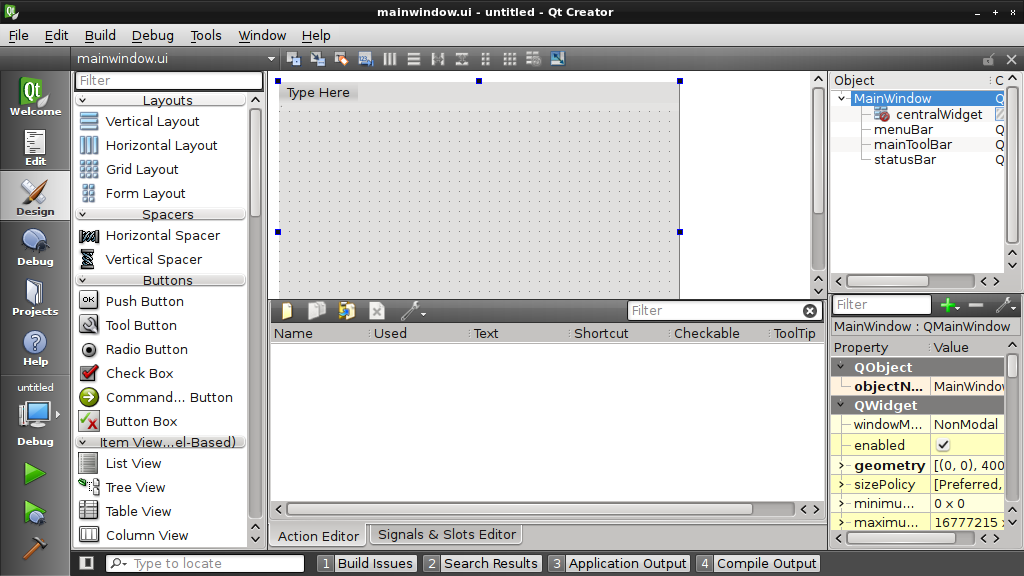
\includegraphics[width=0.9\textwidth]{img/qtcreator}
\end{center}
}

\frame
{
\frametitle{Introducción}
\framesubtitle{Herramientas de Ayuda}
\begin{itemize}
	\item Designer
\end{itemize}
\begin{center}
	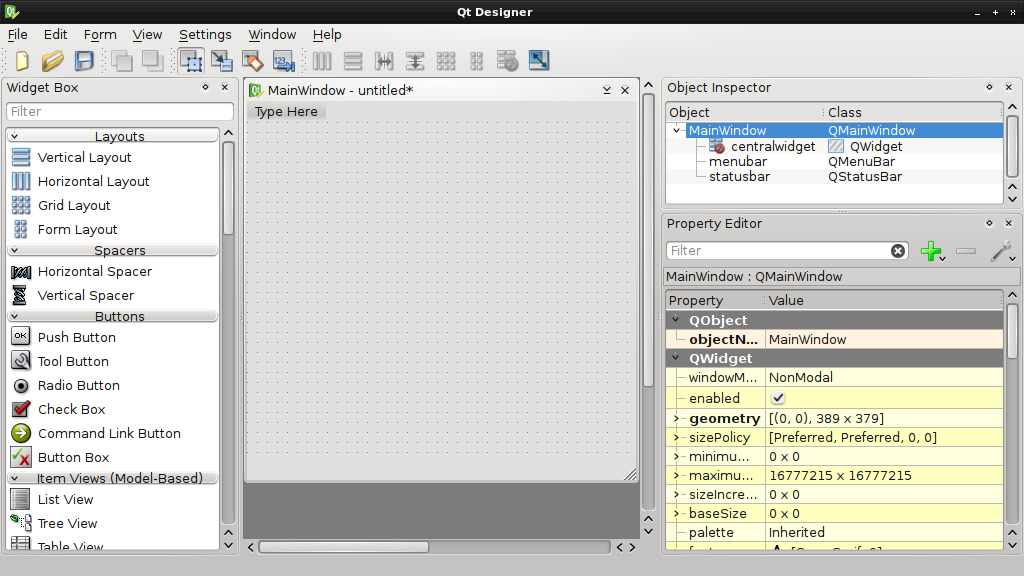
\includegraphics[width=0.9\textwidth]{img/designer}
\end{center}
}

\frame
{
\frametitle{Introducción}
\framesubtitle{Hello World}
\lstset{language=Python}
\lstinputlisting{code/01/hello.py}
}

\frame
{
\frametitle{Introducción}
\framesubtitle{Simple}
\lstset{language=Python}
\lstinputlisting{code/02/simple.py}
}
